\chapter{Disseny de hardware}\label{chapter:disseny de hardware}
En aquest capítol comentarem tot el disseny del hardware que s'ha seguit per poder controlar l'expenedor automàtic assolint els requisits definits anteriorment.

\section{Disseny elèctric}
A partir de l'esquema elèctric simplificat de l'expenedor, la idea del nostre disseny elèctric és d'afegir un circuit paral·lel a la màquina de canvi i als botons de selecció per poder accionar el motor del carril desitjat i que pugui deshabilitar la màquina de canvi durant el transcurs d'una venda en el nostre sistema. 

Per aconseguir deshabilitar la màquina de canvi, afegim un relé commutador abans d'aquesta i així també dirigir el corrent cap els relés que accionaran els motors.

Els relés es connecten en serie de la mateixa manera que els botons de selecció per evitar que més d'un d'ells pugui tancat el circuit al mateix temos.

Per tal de poder controlar l'estat de l'expenedor per saber si no queda producte en algun carril o si la venda ha quedat deshabilitada per algun motiu, s'ha de poder verificar si hi ha tensió en certs punts del circuit.

Per verificar que el carril no està buit i hi queda producte per vendre, es pot observar si la làmpada esta encesa mesurant la tensió que cau entre els seus borns. Això ho farem amb un circuit que hem trobat en un blog\autocite{sensing-circuit} de projectes casolans i hem adaptat al nostre sistema:

Un rectificador d'alta impedància connectat a un opto-acoblador per separar els circuits de l'expenedor dels circuits del nostre hardware.

\begin{figure}[H]
\center
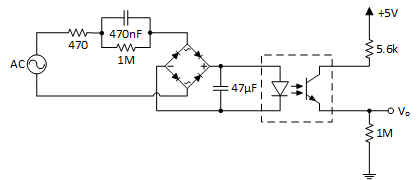
\includegraphics[width=0.8\textwidth]{images/sensing}
\caption{Esquema elèctric del circuit de sensing}
\label{fig:sensing_board}
\end{figure}

Per verificar que la venda no ha quedat deshabilitada, mesurarem la tensió al node comú del relé de by-pass amb el mateix circuit anterior.

\begin{figure}[H]
\center
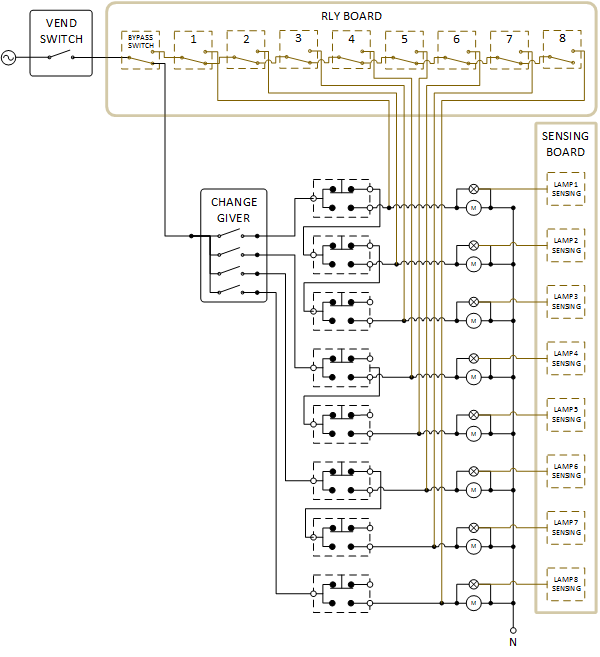
\includegraphics[width=0.8\textwidth]{images/vender_electrical_complete}
\caption{Esquema elèctric proposat de l'expenedor}
\label{fig:vender_electrical_complete}
\end{figure}

Tot i que pel funcionament del nostre sistema no és gaire rellevamt, també mesurarem la tensió a la làmpada de \textit{canvi exacte} per poder notificar al servidor que l'expenedor gairebé s'ha quedat sense canvi.

\section{Components}
Com a controlador central de l'expenedor es farà servir un ordinador de placa petita \textit{RaspberryPi 2 B} (a partir d'ara, RPi), ja que disposa de bastants pins d'entrada/sortida, se li pot instal·lar un sistema operatiu basat en linux (que fa molt més fàcil el disseny de l'aplicació de client), té connexió a internet, possibilitat de connectar-hi una pantalla per HDMI o bé una pantalla tàctil.

Per a la interfície d'usuari usarem la pantalla tàctil \textit{Raspberry Pi Touch 7"}.

Per a poder accionar els circuits que accionen els motors de l'expenedor des de la RPi farem servir una placa de relés activats per nivell baix.

Per a llegir les targetes NFC s'utilitzarà un mòdul NFC PN532, connectat per un adaptador USB a la RPi. S'alimenta a 5V a través de l'adaptador USB.

La RPi necessitarà una alimentació de 5V i 1A.
La pantallà tàctil necessita una alimentació de 5V i 1A.
Els circuits dissenyats anteriorment s'alimenten a 5V.
La placa de relés necessita una alimentació de 12V. Per tant necessitarem una font d'alimentació de 5V i 12V.

\begin{figure}[H]
\center
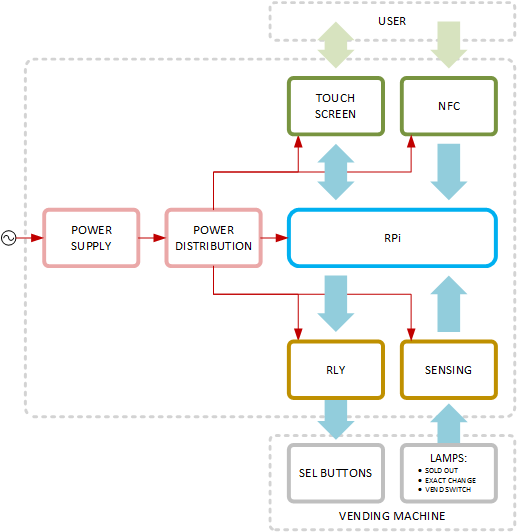
\includegraphics[width=0.8\textwidth]{images/block_diagram}
\caption{Diagrama de bloc de la unitat de test}
\label{fig:block_diagram}
\end{figure}

\section{Unitat de prova}
Per tal de poder fer proves amb el sistema prèvies a la integració final, s'ha desenvolupat una unitat de test que consisteix en una capsa de metacrilat que conté tots els components fixats a dins i interconnectats de manera que sigui fàcil de transportar.

A més, s'ha desenvolupat una placa de sensing a part per a la unitat de test ja que el sensing sobre alta tensió no té gaire sentit fer-lo si no és sobre l'expenedor.

\begin{figure}[H]
\center
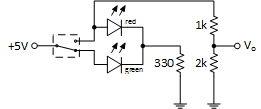
\includegraphics[width=0.8\textwidth]{images/sensing_demonstrator}
\caption{Esquema elèctric del circuit de sensing de la unitat de test}
\label{fig:sensing_demonstrator_board}
\end{figure}

Aquesta placa té uns pins d'entrada on hi van conectats les sortides dels relés i quan s'activa un relé s'encén un LED per poder visualitzar des de fora de la capsa quins relés estan activats.

També té uns polsadors interruptors que són per a simular l'estat de les làmpades dels botons de selecció, que estan connectats als pins de sortida de la placa que aniran connectats als pins d'entrada de la RPi.

\begin{figure}[H]
\center
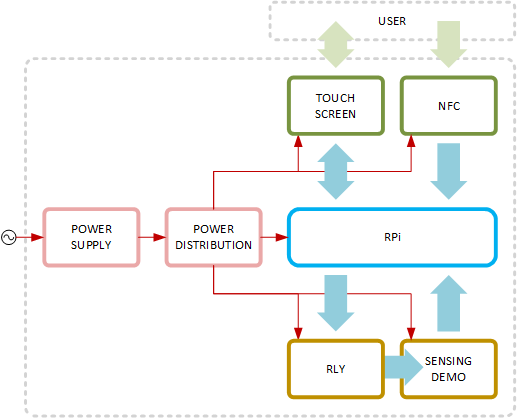
\includegraphics[width=0.8\textwidth]{images/demonstrator_diagram}
\caption{Diagrama de bloc de la unitat de test}
\label{fig:demonstrator_diagram}
\end{figure}